\begin{blocksection}
\question
On the rising edge of the clock, B is set to A and is held constant until the next rising edge.  Fill in the diagram for B’s value.

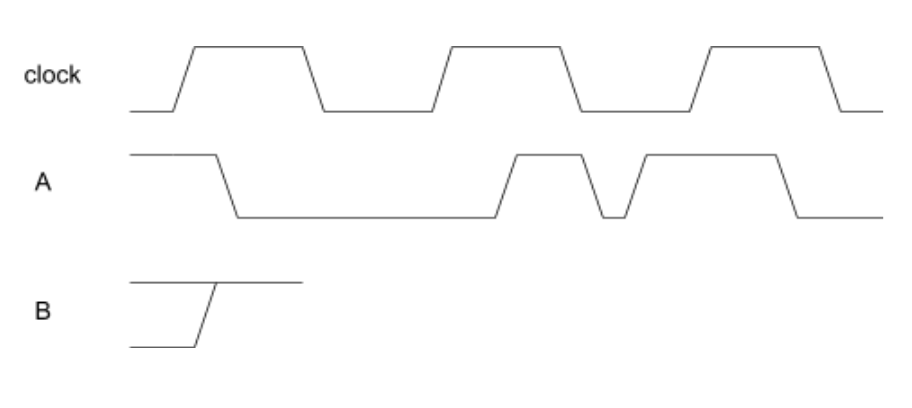
\includegraphics[width=\textwidth]{sds/basics_a}
\begin{solution}
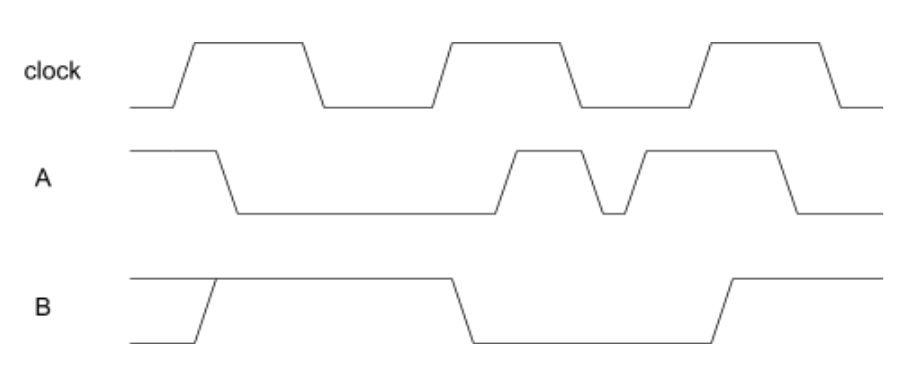
\includegraphics[width=\textwidth]{sds/basics_a_sol}
\end{solution}

In a clock cycle, complex operations can occur.  For example, most of the RISC-V instructions can be done in 1 clock cycle.  Below, the diagram shows the equation Z = X + Y where Z is computed on the rising edge of the clock.  If Z overflows, place the overflow in the carry bit.

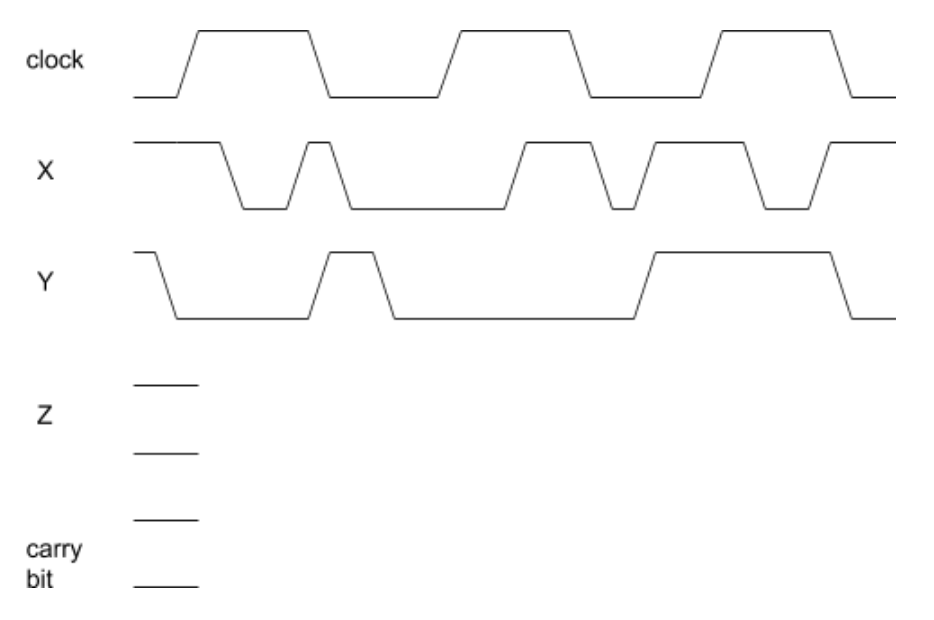
\includegraphics[width=\textwidth]{sds/basics_b}
\begin{solution}
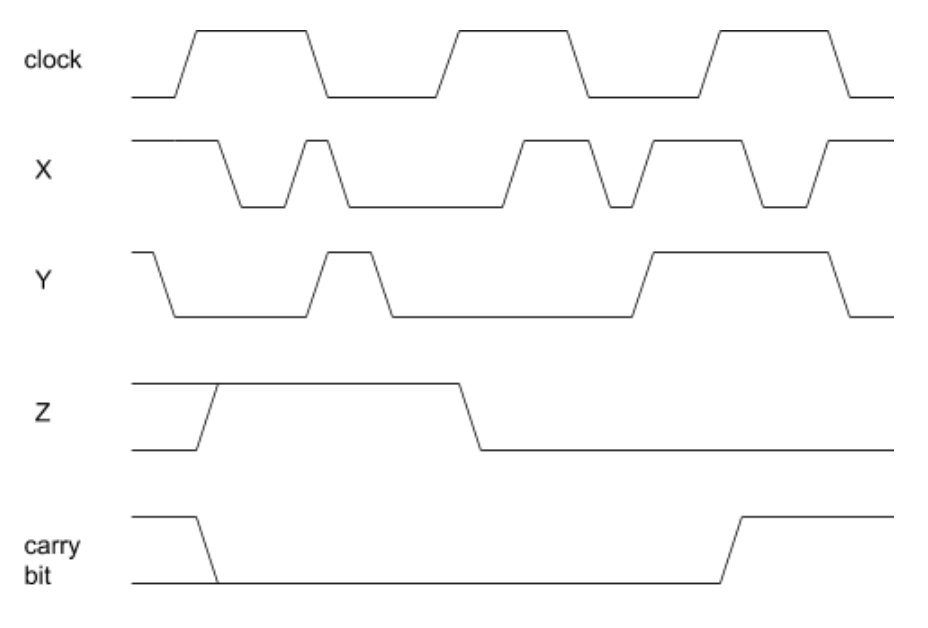
\includegraphics[width=\textwidth]{sds/basics_b_sol}
\end{solution}

\end{blocksection}